\section{Literature Review}
\label{sec:formatting}

%-------------------------------------------------------------------------
\subsection{Bootstrapping Language-Image Pre-training}
The BLIP model architecture (see Fig. 2) proposed by Li et. al \cite{li2022blip}, is a new Vision-Language Pretraining framework that achieves state-of-the-art performance on various vision-language tasks by addressing the limitations of existing methods. BLIP utilises a new dataset bootstrapping technique called CapFilt, which generates synthetic captions and filters out noisy captions to improve the quality of the dataset. The proposed framework introduces a multimodal mixture of encoder-decoder (MED) model architecture and leverages pre-training objectives such as image-text contrastive learning, image-text matching, and image-conditioned language modelling to achieve flexible transfer learning and effective multi-task pre-training.

\begin{figure}[htbp]
  \centering
   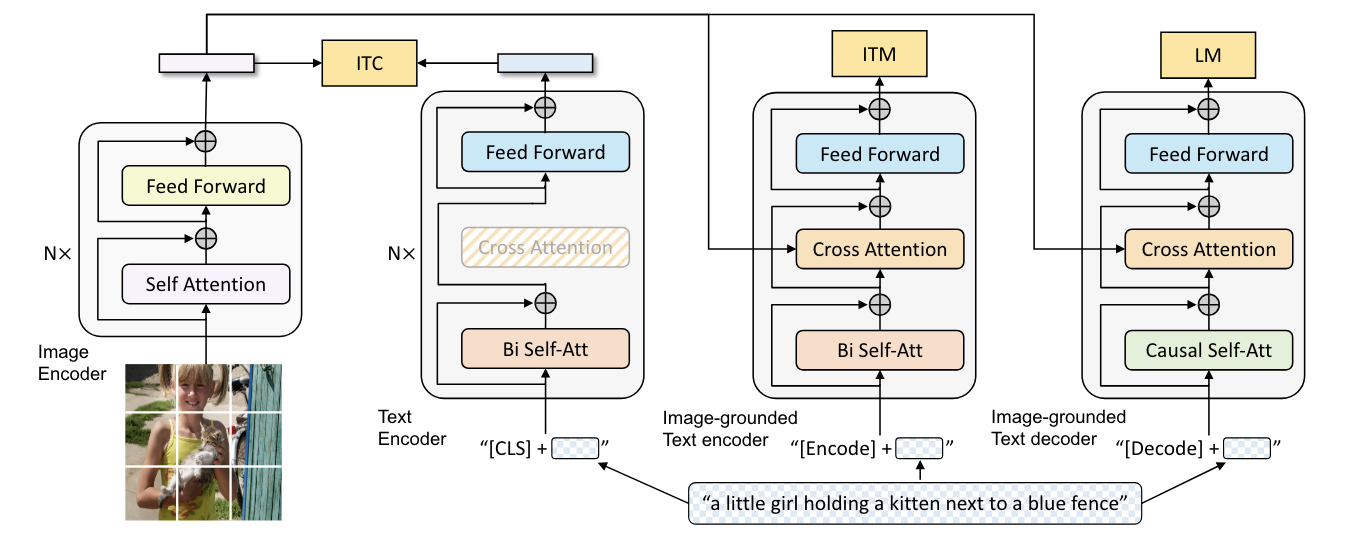
\includegraphics[width=\linewidth]{sec/Images/image2.png}
   \caption{BLIP Architecture}
   \label{fig:onecol}
\end{figure}

%-------------------------------------------------------------------------
\subsection{Wu-Palmer Similarity Score}

In paper by Malinowsk et. al \cite{malinowski2014multi} introduces a performance measure called the WUPS score for evaluating the quality of system-generated answers. It draws inspiration from Fuzzy Sets theory and utilises the Wu-Palmer Similarity (WUPS) score to account for semantic fuzziness between classes. WUPS score penalises both underestimation and overestimation of answers. The formula considers the intersection of system and ground-truth answers, employing a soft membership measure. Empirical findings suggest a WUP score of approximately 0.9 for precise answers, prompting down-weighting for scores below a threshold. A curve over thresholds illustrates the trade-off between precision and forgiveness, with WUPS at 0 being the most lenient measure and WUPS at 1.0 equating to standard accuracy. Further details about the evaluation metric will be discussed in the subsequent sections. 


%-------------------------------------------------------------------------
% \subsection{References}

% List and number all bibliographical references in 9-point Times, single-spaced, at the end of your paper.
% When referenced in the text, enclose the citation number in square brackets, for
% example~\cite{Authors14}.
% Where appropriate, include page numbers and the name(s) of editors of referenced books.
% When you cite multiple papers at once, please make sure that you cite them in numerical order like this \cite{Alpher02,Alpher03,Alpher05,Authors14b,Authors14}.
% If you use the template as advised, this will be taken care of automatically.

% \begin{table}
%   \centering
%   \begin{tabular}{@{}lc@{}}
%     \toprule
%     Method & Frobnability \\
%     \midrule
%     Theirs & Frumpy \\
%     Yours & Frobbly \\
%     Ours & Makes one's heart Frob\\
%     \bottomrule
%   \end{tabular}
%   \caption{Results.   Ours is better.}
%   \label{tab:example}
% \end{table}

% %-------------------------------------------------------------------------
% \subsection{Illustrations, graphs, and photographs}

% All graphics should be centered.
% In \LaTeX, avoid using the \texttt{center} environment for this purpose, as this adds potentially unwanted whitespace.
% Instead use
% {\small\begin{verbatim}
%   \centering
% \end{verbatim}}
% at the beginning of your figure.
% Please ensure that any point you wish to make is resolvable in a printed copy of the paper.
% Resize fonts in figures to match the font in the body text, and choose line widths that render effectively in print.
% Readers (and reviewers), even of an electronic copy, may choose to print your paper in order to read it.
% You cannot insist that they do otherwise, and therefore must not assume that they can zoom in to see tiny details on a graphic.

% When placing figures in \LaTeX, it's almost always best to use \verb+\includegraphics+, and to specify the figure width as a multiple of the line width as in the example below
% {\small\begin{verbatim}
%    \usepackage{graphicx} ...
%    \includegraphics[width=0.8\linewidth]
%                    {myfile.pdf}
% \end{verbatim}
% }


% %-------------------------------------------------------------------------
% \subsection{Color}

% Please refer to the author guidelines on the \confName\ \confYear\ web page for a discussion of the use of color in your document.

% If you use color in your plots, please keep in mind that a significant subset of reviewers and readers may have a color vision deficiency; red-green blindness is the most frequent kind.
% Hence avoid relying only on color as the discriminative feature in plots (such as red \vs green lines), but add a second discriminative feature to ease disambiguation.